\section{Introduction}

%llm
Large language models (LLMs) have reshaped AI research and implementations, with unprecedented capabilities widely shown in various language-related tasks \cite{achiam2023gpt, leiter2024chatgpt, reid2024gemini, adler2024nemotron, jiang2023mistral, touvron2023llama, team2024gemma}, bringing humans ever close to general AI \cite{brown2020language, bubeck2023sparks, ge2024openagi}.
Recent research on multi-agent systems has further magnified LLMs' advantages of {\textit{broad knowledge}, \textit{language comprehension}, and \textit{generalizability}} through conversational collaborations, showing strong promise for further human-model collaboration for critical applications \cite{bankes2002agent, bai2022constitutional, bonabeau2002agent, li2023camel, wu2024autogen}.
Recent studies have also revealed the limitations of LLMs regarding their {\textit{lack of planning} \cite{hu2023large, mousavi2024your, yadkori2024believe, asai2024selfrag,yu2024rankrag}, \textit{fuzzy inference} \cite{liu2023evaluating, zhu2023dyval, zhuo2024roles, yuan2024back, wang2023boosting}, and \textit{hallucination} \cite{ji2023survey, bai2024hallucination, tonmoy2024comprehensive, maynez2020faithfulness, xiao2021hallucination, farquhar2024detecting, ji2023towards, chen2024inside}}. Specifically, in many real-world application scenarios, the lack of accurate planning can be caused by the lack of access to high-quality domain knowledge, especially the rapidly evolving new knowledge; the fuzzy inference nature can lead to difficulties in conducting reliable comprehension and stable predictions for complex questions; and hallucination creating factual errors and misinformation can cause fatal and life-threatening problems in critical applications \cite{wornow2023shaky, shen2023chatgpt, pal2023med, xu2024simrag, panagoulias2024evaluating, gu2024medvh}.
% motivations for multi-agent systems, black-box nature of LLMs makes it hard to share data/resource

%kg
Knowledge graphs (KGs) have been widely studied across academia and industry, due to their advantages in {\textit{storing accurate knowledge}, \textit{facilitating explicit inference}, and \textit{allowing easy editing of the knowledge} \cite{hogan2021knowledge, ji2021survey, wang2017knowledge, zou2020survey}}.
{However, the creation of KGs relies much on the \textit{standardization of data}, which requires significant schematic designs and human efforts.}
In many application domains, researchers and professionals have spent decades collecting, processing, and curating various types of data towards the construction of KGs \cite{cui2023review, su2023biomedical, cornet2008forty, santos2020clinical, harrison2021icd, lipscomb2000medical, bodenreider2004unified, xu2020building, li2020real, lv2023tcmbank}, which are widely used to support downstream application such as search and ranking \cite{xiong2017explicit, liu2018entity, vu2019capsule}, user modeling and recommendation \cite{wang2019kgat, wang2021learning, yang2022knowledge}, basic science research \cite{feng2023genomickb, shao2022knowledge, quan2023aimedgraph, zhang2021discovering, li2022prediction, jeong2022intelligent}, healthcare \cite{xu2023seqcare,jiang2024graphcare,xu2024ram} and education \cite{chen2018knowedu, rizun2019knowledge}. 
{Nevertheless, KGs still suffer from \textit{incomplete knowledge coverage}, due to the stringent requirements on data standardization and limited data volumes compared to unstructured data in the wild, while specific algorithms are often needed to fill \textit{their gaps to applications}}.
Moreover, real-world data are noisy and complex, where entities and relations come from various sources such as institutions using different data schemas and naming conventions \cite{tang2022intelligent, yuan2012multi, zhang2010multi}, and the data can also include multiple modalities such as tables, texts, images, and time series \cite{huang2021makes, baltruvsaitis2018multimodal, acosta2022multimodal, cai2019survey, zhang2022m3care, soenksen2022integrated, shaik2023survey, krones2024review, cremonesi2023need, iakovidis2012semantic, kline2022multimodal, stahlschmidt2022multimodal}. 
While such multi-source and multi-modality data hold great promise in integrative and comprehensive analysis, unifying and extracting high-quality knowledge from them is non-trivial.

\begin{figure}[t]
\centering
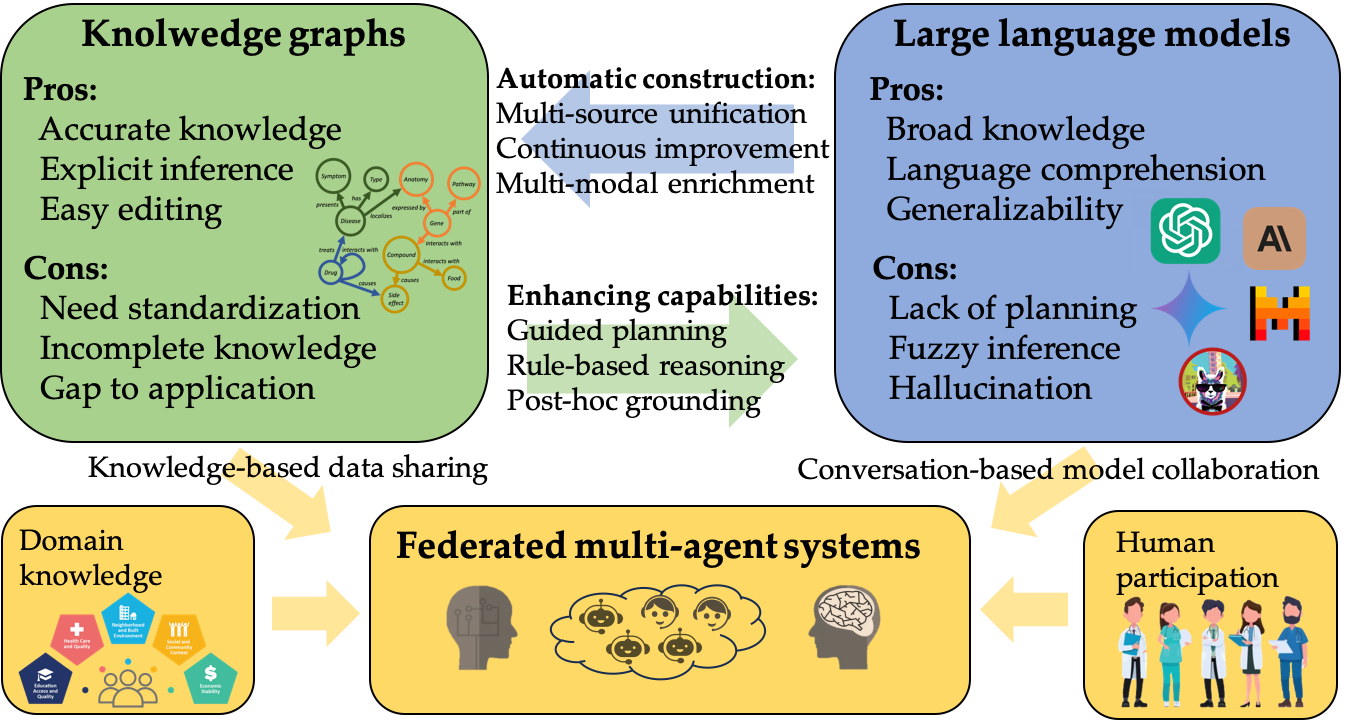
\includegraphics[width=30pc]{submissions/CarlYang2024/figures/intro.png}
\vspace{-3mm}
\caption{Overview of the proposed {knowledge graph and large language model co-learning framework}.}
\vspace{-5mm}
\label{fig:intro}
\end{figure}

%kg+llm existing combinations and limitations
%synergized modeling: roadmap
%KG for LLM: new knowledge, knowledge representation, interpretation-- do not rigorously address the unique challenges in healthcare
%LLM for KG: embedding, completion, construction-- do not comprehensively handle the unique challenges in healthcare
%LLM+KG for health: specific applications without fundamentally improving LLMs and KGs for healthcare
%multi-agent: role play-- do not consider the unique challenges in healthcare regarding privacy, values and disparity
Recently, significant research attention has been drawn to the synergies between KGs and LLMs \cite{pan2023large, pan2024unifying, pan2024integrating, wang2021kepler, yu2022jaket, yasunaga2022deep, jiang2024efficient}, due to their naturally complementary advantages (Figure \ref{fig:intro}). 
The construction and modeling of KGs have often relied on advances in natural language processing (NLP), with recent efforts intensively exploring language models towards the embedding \cite{wang2022language, yu2022cocodr, xie2023lambdakg, choudhary2023complex, zhang2020pretrain, ke2021jointgt}, completion \cite{yao2019kg, kim2020multi, lv2022pre, shen2022joint, choi2023knowledge, wang2021structure, wang2022simkgc, li2023multi, saxena2022sequence, chen2022knowledge, chen2023dipping, lovelace2022framework, xie2022discrimination} and construction \cite{zhu2023llms, ye2022generative, qin2023chatgpt, kommineni2024human, zhang2024extract, vizcarra2024representing, yu2023bear, hu2023llm, meyer2023llm, hofer2024towards, yang2024graphusion, melnyk2021grapher, kumar2020building, chen2022knowprompt, wan2023gpt, wang2024kglink, li2024preliminary, yan2021unified, ding2022prompt, efeoglu2024retrieval, li2022ultra, ayoola2022refined, cattan2021cross, thirukovalluru2021scaling, alt2019improving, guo2021constructing, bosselut2019comet, hao2022bertnet, west2022symbolic} of KGs. 
Studies in the recent years have also bloomed to explore the utilization of KGs for enhancing LLMs through providing new sources of knowledge during pre-training \cite{hu2023survey, wei2021knowledge, yin2022survey, wang2023unifying, sun2022jointlk, liu2021kg, qi2021answering, mavromatis2024gnn, zhang2022greaselm, feng2020scalable, yasunaga2021qa, zhang2019ernie, sun2021ernie, liu2020k, dai2022knowledge, shen2020exploiting, zhang2020bert, tian2020skep, rosset2020knowledge, li2022pre, xiong2020pretrained, he2020bert, su2021cokebert, zhu2023pre, feng2023knowledge, huang2022endowing, agarwal2021knowledge, xu2023kilm, oguz2022unik, tan2024walklm, xu2024bmretriever,sun2020colake, zhang2022dkplm, ye2022ontology, luo2023chatkbqa, martino2023knowledge, chen2020kgpt, santos2022knowledge, moiseev2022skill} or inference \cite{li2023graph, jiang2023unikgqa, luo2024reasoning, sun2024think, wang2024reasoning, luo2023chatrule, wang2023enhancing, besta2024graph, wang2019improving, wang2024knowledge, allemang2024increasing, ji2023rho, feng2023factkb, mcdonald2024reducing, lee2022promptiverse, brate2022improving, wen2023mindmap, wilmot2021memory, logan2019barack, wu2022efficient, guan2024mitigating, dong2024don, sarthi2024raptor, he2024g, han2023pive, edge2024local, gutierrez2024hipporag, liang2024empowering}, and enabling knowledge-based interpretation and evaluation \cite{petroni2019language, jiang2020can, adolphs2021query, shin2020autoprompt, mallen2022not, cohen2023qa, luo2023systematic, liu2023evaluating, orogat2021cbench, zhu2023dyval, bai2024kgquiz, ho2020constructing}. 
Finally, pioneering studies have also been conducted to explore LLM-based multi-agent systems, mostly through prompt-based role-plays to simulate human collaborations \cite{tracy2018agent, tang2024medagents, kaur2024llm, li2024agent, kim2024adaptive, gebreab2024llm, yue2024ct, pan2024agentcoord, xiao2024cellagent}. 

{In this paper, we re-emphasize the promise of KG and LLM co-learning, especially through a structure-oriented retrieval augmented generation (SRAG) paradigm, where LLMs extract structured knowledge from unstructured data, which can be further retrieved to enhance the capabilities and reliabilities of LLMs during applications.}
Specifically, we give examples and discuss several natural and promising use cases where LLMs can be utilized to automate the construction of high-quality KGs. Furthermore, we summarize and highlight several limitations of current LLMs that can be potentially mitigated through the utilization of KGs. Finally, we envision a federated multi-agent system where models and data are disentangled while humans and knowledge are deeply engaged. Future directions are further discussed in the end.